\documentclass[12pt, a4paper]{article}

% --- Packages ---
\usepackage[margin=2.5cm]{geometry}
\usepackage{setspace}
\usepackage{booktabs}
\usepackage{array}
\usepackage{longtable}
\usepackage{hyperref}
\usepackage[dvipsnames]{xcolor}
\usepackage{titlesec}
\usepackage{fancyhdr}
\usepackage{graphicx}
\usepackage{amsmath}
\usepackage{amssymb}
\usepackage{enumitem}
\usepackage{parskip}
\usepackage[T1]{fontenc}
\usepackage{lmodern}
\usepackage[polish]{babel}
\usepackage[utf8]{inputenc}
\usepackage[backend=biber, style=numeric, sorting=nyt]{biblatex}

\addbibresource{references.bib}
\addto\captionspolish{
    \renewcommand{\figurename}{Rycina}
}
% --- Hyperref setup ---
\hypersetup{
    colorlinks = true,
    linkcolor  = blue!60!black,
    citecolor  = blue!60!black,
    urlcolor   = blue!60!black
}

% --- Header/Footer ---
\pagestyle{fancy}
\fancyhf{}
\rhead{\textit{Plan Analizy Statystycznej}}
\lhead{
\includegraphics[scale=0.2]{graphics/logo-i-orzel.png}}
\rfoot{Strona \thepage}
\lfoot{\textit{}}

% --- Section formatting ---
\titleformat{\section}{\large\bfseries}{{\thesection}}{1em}{}[\titlerule]
\titleformat{\subsection}{\normalsize\bfseries}{{\thesubsection}}{1em}{}

% --- Custom commands ---
\newcommand{\placeholder}[1]{\textcolor{red!70!black}{[#1]}}
\newcommand{\TODO}[1]{\textcolor{orange!80!black}{\textbf{TODO:} #1}}

% ============================================================
\begin{document}
% ============================================================

% --- Strona tytułowa ---
\begin{titlepage}
    \centering
    \vspace*{2cm}
    {\LARGE \textbf{Plan Analizy Statystycznej} \par}
    \vspace{0.5cm}
    {\large Bayesowska analiza przeżycia róż: ocena skuteczności związków chemicznych w fazie pilotażowej i badaniu głównym\par}
    \vspace{2cm}
    \centering
    
\includegraphics[width=0.3\textwidth]{graphics/UMB-logo.png}\par\vspace{2cm}

    \begin{tabular}{ll}
        \toprule
        \textbf{Wersja dokumentu}  & 1.0 \\
        \textbf{Data}              & \today \\
        \textbf{Autorzy}         & Julia Czyż, Urszula Skuńczyk, Paulina Włodarczyk\\
        \textbf{Afiliacja}         & Uniwersytet Medyczny w Białymstoku \\
                                   & Zakład Biostatystyki i Informatyki Medycznej \\

        \bottomrule
    \end{tabular}

    \vspace{2cm}
    \vfill
\end{titlepage}

% --- Spis treści ---
\tableofcontents
\newpage

\onehalfspacing

% ============================================================
\section{Wprowadzenie}
% ============================================================

\subsection{Tło badania}
Jean-Baptiste de la Tour Fleurie jest botanikiem mieszkającym w zamku w niewielkim mieście Farmac, położonym niedaleko portu La Rochelle. Jest romantykiem oraz miłośnikiem pięknych kwiatów. W ogrodach swego zamku z pasją i szczególnym zaangażowaniem zajmował się hodowlą róż, które były oczkiem w jego głowie. Pewnego dnia odkrył jednak coś znacznie cenniejszego niż dotychczasowa radość płynąca z obserwacji jego ukochanych roślin. Poznał kobietę, w jego oczach piękniejszą niż najpiękniejsze z jego róż i zakochał się w niej. Wielokrotnie obdarowywał ją kwiatami, lecz jego starania nie przyniosły efektu. Rodzice owej panny przysięgli oddać jej rękę jedynie temu, który ofiaruje jej najrzadszy ze skarbów -- czarnego tulipana. Większość śmiałków przekonana była, że kwiat ten istnieje wyłącznie w legendach, jednak Jean-Baptiste dokładnie wiedział, gdzie można go znaleźć. Czczony niczym bóstwo czarny tulipan rósł na niewielkim archipelagu na Oceanie Atlantyckim. Jedynym sposobem na zdobycie kwiatu było ścięcie go, ponieważ tubylcy zamieszkujący wyspy nie pozwalali go wykopać. Botanik nie wiedział jednak, w jaki sposób przetransportować kwiat do portu w La Rochelle, tak aby zachował świeżość i mógł zostać ofiarowany ukochanej.

\par Podróż statkiem trwa zazwyczaj około 10 dni, jednak w zależności od warunków pogodowych może trwać od 8 do 22 dni. Jean-Baptiste, nie mając doświadczenia w utrzymywaniu ściętych kwiatów przy życiu, rozesłał listy w nadziei na znalezienie pomocy, której tak desperacko potrzebował.
\par Ponieważ czarny tulipan jest wyjątkowo rzadki, badanie prowadzone jest na różach dwóch odmian: \textit{T.~floribunda} oraz \textit{T.~hybrid}, pochodzących z ogrodów Jean-Baptiste’a, które udostępnił na potrzeby przeprowadzenia eksperymentów. Głównym celem jest znalezienie sposobu na przewiezienie czarnego tulipana w nienaruszonym stanie, umożliwiając Jean-Baptiste’owi zdobycie ręki ukochanej.

\subsection{Cele badania}
Głównym celem badania jest identyfikacja związku chemicznego, który zapewni najdłuższy czas przeżycia kwiatu podczas transportu morskiego. W tym celu związki uporządkowane zostaną według mediany czasu przeżycia wyestymowanej z bayesowskiego modelu przeżycia.

Cele drugorzędowe obejmują:
\begin{itemize}[noitemsep]
    \item Estymację mediany czasu przeżycia oraz przedziału wiarygodności dla każdego z badanych związków.
    \item Ocenę prawdopodobieństwa przeżycia kwiatu przez typowy czas podróży wynoszący 10 dni dla każdego związku.
    \item Ocenę prawdopodobieństwa przeżycia kwiatu przez maksymalny czas podróży wynoszący 22 dni dla każdego związku.
\end{itemize}

\subsection{Punkty końcowe i kryteria decyzyjne}\label{subsec:endpoints}

\textbf{Pierwszorzędowy punkt końcowy:}
\par Ranking związków według mediany czasu przeżycia $\exp(\beta_0 + \alpha_c) \cdot (\ln 2)^{1/k}$ wyznaczonej z rozkładu a posteriori. Związek z najwyższą medianą uznany zostanie za najlepszy.\\
\textbf{Drugorzędowe punkty końcowe:}
\begin{itemize}[noitemsep]
    \item Estymację prawdopodobieństwa przeżycia kwiatu przez typowy czas podróży ($t = 10$ dni) dla każdego związku, wyznaczoną jako uśrednioną po próbkach a posteriori wartość funkcji przeżycia:
    \[
        \hat{S}_c(10) = \frac{1}{S}\sum_{s=1}^{S} \exp\!\left[-\!\left(\frac{10}{\lambda_c^{(s)}}\right)^{\!k^{(s)}}\right], \quad \lambda_c^{(s)} = \exp\!\left(\beta_0^{(s)} + \alpha_c^{(s)}\right)
    \]
    \item Estymację prawdopodobieństwa przeżycia kwiatu przez maksymalny czas podróży ($t = 22$ dni) dla każdego związku, wyznaczoną analogicznie jako $\hat{S}_c(22)$, zakładając możliwie najgorsze warunki pogodowe.
\end{itemize}

\subsection{Zakres PAS}
Niniejszy Plan Analizy Statystycznej obejmuje analizę eksploracyjną danych pilotażowych oraz szczegółowy opis zaplanowanej analizy głównej. Dokument został sfinalizowany przed ujawnieniem głównych danych.

% ============================================================
\section{Schemat badania}
% ============================================================

\subsection{Projekt badania}\label{experiment:scheme}
\indent Jednostki eksperymentalne podzielono na cztery równoliczne bloki, aby kontrolować wpływ warunków środowiskowych, w jakich były hodowane, uwzględniając przy tym różnorodność gatunkową kwiatów (\texttt{species}) oraz ich pochodzenie (\texttt{garden}). Zbierano rośliny możliwie jak najbardziej zbliżone do siebie pod względem stadium rozwoju, czy cech wyglądu. Każdą z piętnastu analizowanych substancji rozpuszczono oddzielnie w wodzie, otrzymując roztwory o identycznych stężeniach. Następnie, w obrębie każdego bloku, róże losowo podzielono na piętnaście równych podgrup, z których każdą przypisano do jednego roztworu, w którym kwiaty pozostawały zanurzone przez cały czas trwania eksperymentu, tj. 30 dni. Róże umieszczono w specjalnie przygotowanym na potrzeby eksperymentu laboratorium, gdzie zapewniono im stabilne warunki środowiskowe, takie jak temperatura i wilgotność powietrza, zbliżone do warunków występujących pod pokładem statku. Celem tego zabiegu było wyeliminowanie potencjalnych różnic w czasie przeżycia kwiatów, spowodowanych niestabilnymi parametrami otoczenia oraz symulacja warunków, w jakich docelowo przywożony ma być czarny tulipan. Kwiatów raz umieszczonych w płynie, nie wyjmowano aż do momentu wystąpienia zdarzenia, będącego podmiotem tej analizy -- obumarcia rośliny. Każdego dnia trwania eksperymentu w równych odstępach czasowych, ogrodnicy dokonywali oceny kwiatów, jednoznacznie stwierdzając czy dany okaz nadal jest wizualnie zadowalający. Szczegóły na temat rodzaju roztworu, w którym zanurzone były poszczególne kwiaty nie zostały im ujawnione. Opisany schemat odnosi się do badania pilotażowego, w którym uwzględniono wszystkie piętnaście substancji. W badaniu głównym, na podstawie wyników analizy eksploracyjnej danych pilotażowych, związki 2, 3 oraz 10 zostały wykluczone -- szczegółowe uzasadnienie przedstawiono w Sekcji~\ref{subsec:cloglog}.

\subsection{Jednostki eksperymentalne}
Jednostką eksperymentalną jest pojedynczy okaz róży (\texttt{id}), pochodzącej z jednego z dwóch ogrodów (\texttt{garden}) i należący do jednego z dwóch dostępnych gatunków (\texttt{species}).

\subsection{Grupy interwencji}
W badaniu pilotażowym uwzględniono piętnaście substancji (związki 1--15), których pełną listę przedstawiono w Tabeli~\ref{tab:compounds}. Na podstawie analizy eksploracyjnej danych pilotażowych podjęto decyzję o wykluczeniu związków 2, 3 oraz 10 z badania głównego (uzasadnienie w Sekcji~\ref{subsec:cloglog}). W badaniu głównym analizie poddanych zostanie zatem dwanaście substancji: związek 1 jako grupa kontrolna oraz związki 4--9 i 11--15 jako grupy interwencji.

\begin{longtable}{cl}
\caption{Identyfikatory i nazwy związków chemicznych}
\label{tab:compounds}\\
\toprule
\textbf{ID} & \textbf{Nazwa związku} \\
\midrule
\endfirsthead
\toprule
\textbf{ID} & \textbf{Nazwa związku}  \\
\midrule
\endhead
\bottomrule
\endfoot
1  & Distilled Water           \\
2  & Apathic Acid              \\
3  & Beerse Brew               \\
4  & Concentrate of Caducues   \\
5  & Distillate of Discovery   \\
6  & Essence of Epiphaneia     \\
7  & Four in December          \\
8  & Granules of Geheref       \\
9  & Kar-Hamel Mooh            \\
10 & Lucifer's Liquid          \\
11 & Noospherol                \\
12 & Oil of John's Son         \\
13 & Power of Perlimpinpin     \\
14 & Spirit of Scienza         \\
15 & Zest of Zen               \\
\end{longtable}

\subsection{Definicja punktu końcowego}
Głównym punktem końcowym był \textbf{czas przeżycia} (\texttt{time}), zdefiniowany jako liczba dni od rozpoczęcia eksperymentu, tj. umieszczenia roślin w roztworach, do wystąpienia zdarzenia (obumarcie/więdnięcie, równoznaczne z utratą pożądanych walorów estetycznych). Pomiarów dokonywano z dokładnością do jednego dnia, stąd zmienna \texttt{time} przyjmuje wartości całkowite z przedziału [0, 30], gdzie dzień 0 oznacza początek eksperymentu (dzień zanurzenia kwiatów w roztworach), a właściwa obserwacja obejmuje dni od 1 do 30.

Wskaźnik zdarzenia \texttt{can.be.presented} dostarcza informacji o walorach estetycznych róży. W dniu eksperymentu, w którym wygląd kwiatu przestawał być zadowalający zmienna przyjmowała wartość \texttt{FALSE}, co oznaczało wystąpienie zdarzenia i zakończenie obserwacji dla danej jednostki. Natomiast w przypadku kwiatu, który w ostatnim, trzydziestym dniu eksperymentu nadal nadawał się do prezentacji, zmienna przyjmowała wartość \texttt{TRUE}, co oznaczało obserwację prawostronnie cenzurowaną.

\subsection{Liczebność próby}
W badaniu głównym zaplanowano wykorzystanie łącznie około dwóch tysięcy jednostek eksperymentalnych, co wynika z maksymalnej liczby kwiatów dostępnych na potrzeby eksperymentu, zadeklarowanej przez ogrodników. Przy przyjętym blokowym układzie eksperymentu obejmującym 12×2×2=48 komórek eksperymentalnych założono równomierne rozłożenie próby, co odpowiada około 40 kwiatom na każdą komórkę.
\par Przeprowadzone badanie pilotażowe obejmowało 15 kwiatów na każdą komórkę. Zwiększenie liczebności do 40 ($\sim 2{,}7$-krotnie) umożliwi uzyskanie przedziałów wiarygodności dla efektów związków $\alpha_c$ węższych o czynnik $\sqrt{2{,}7} \approx 1{,}6$ w porównaniu z danymi pilotażowymi.
% ============================================================
\section{Opis danych}
% ============================================================
W ramach przygotowania niniejszego dokumentu przeprowadzono analizę eksploracyjną danych z badania pilotażowego, które stanowiły odpowiednik docelowego zbioru danych pod względem struktury zmiennych i schematu eksperymentu, z tą różnicą, że obejmował wszystkie piętnaście związków, podczas gdy badanie główne uwzględnia dwanaście. Dane te wykorzystano w celu weryfikacji poprawności zaplanowanej struktury i definicji zmiennych, identyfikacji rozkładów a priori wykorzystywanych w modelach bayesowskich oraz podjęcia decyzji o wykluczeniu związków szkodliwych z badania głównego. Służyły one również do sprawdzenia założeń dotyczących planowanych metod analizy.
\subsection{Struktura zbioru danych (surowych)}
W Tabeli \ref{tab:raw_data_variables} przedstawiono strukturę surowych danych. Ze względu na przyjęty schemat badania (codzienne pomiary) dane miały charakter longitudinalny, gdzie dla każdej obserwacji liczba wierszy odpowiadała liczbie dni przeżycia kwiatu w roztworze, włączając w to dzień 0, czyli dzień rozpoczęcia eksperymentu. 
\begin{longtable}{llp{7cm}}
\caption{Opis zmiennych w danych surowych}\\
\label{tab:raw_data_variables}\\
\toprule
\textbf{Zmienna} & \textbf{Typ} & \textbf{Opis} \\
\midrule
\endfirsthead
\toprule
\textbf{Zmienna} & \textbf{Typ} & \textbf{Opis} \\
\midrule
\endhead
\bottomrule
\endfoot
\texttt{id}                & identyfikator & Unikalny identyfikator róży \\
\texttt{garden}            & kategoryczna & Ogród, z którego pochodzi róża \newline (1~-- Ogród południowy, 2~-- Ogród północny)\\
\texttt{species}           & kategoryczna & Gatunek róży \newline (1~-- \textit{T.~floribunda}, 2~-- \textit{T.~hybrid})\\
\texttt{compound}          & kategoryczna & Przypisany roztwór (1--15) \\
\texttt{time}              & ciągła & Czas przeżycia w dniach (0--30) \\
\texttt{diam}              & ciągła & Średnica kwiatostanu w momencie pomiaru, w centymetrach\\
\texttt{can.be.presented}  & binarna & Wskaźnik wystąpienia zdarzenia\\
\end{longtable}


\subsection{Traktowanie zmiennej czasowej}
Czas przeżycia (\texttt{time}) traktowano jako zmienną \textbf{ciągłą} w całej analizie. Pomimo dokonywania codziennych pomiarów w równych odstępach czasu, co skutkowało uzyskaniem wartości całkowitoliczbowych omawianej zmiennej, badany proces (wystąpienie zdarzenia w badanym czasie) ma naturę ciągłą. Z tego względu przyjęcie ciągłych rozkładów czasu przeżycia jednostek eksperymentalnych jest uzasadnione.

\subsection{Cenzurowanie obserwacji}
Cenzurowanie obserwacji w badaniu miało charakter administracyjny, wynikający z założonego czasu trwania badania. Kwiaty, które ostatniego (30 dnia) trwania eksperymentu nadal zachowały dostateczną świeżość i walory estetyczne, traktowano jako obserwacje prawostronnie cenzurowane (wartość zmiennej \texttt{can.be.presented} = \texttt{TRUE}, przy zmiennej \texttt{time} = 30). Mechanizm cenzurowania był niezależny od czasu przeżycia, ponieważ decyzja o zakończeniu badania podjęta była przed jego rozpoczęciem i nie zależała od stanu kwiatów. W badaniu pilotażowym zaobserwowany odsetek jednostek cenzurowanych wyniósł 0\% (we wszystkich 900 rekordach zdarzenie wystąpiło w trzydziestodniowym okresie badania). 

\subsection{Przetwarzanie danych pilotażowych}\label{sec:pilot_data_processing}
Surowe dane pilotażowe miały strukturę longitudinalną, uwzględniającą codzienne pomiary zmiennych, aż do momentu wystąpienia zdarzenia, bądź zakończenia eksperymentu. W celu dostosowania ich do przyjętej metodologii przekształcono je do postaci, w której na jedną jednostkę eksperymentalną (różę) przypada jedna obserwacja. Zachowano wyłącznie ostatni zarejestrowany pomiar, który zawierał informację o czasie przeżycia (\texttt{time}) oraz statusie jednostki na końcu obserwacji (\texttt{can.be.presented}). Pomiary pośrednie zostały wykluczone z dalszej analizy. Dodatkowo dla każdej jednostki eksperymentalnej utworzono nową zmienną \texttt{baseline\_diam}, która odpowiadała średnicy kwiatostanu w dniu rozpoczęcia eksperymentu. Na potrzeby eksploracyjnej analizy danych wprowadzono pomocniczy podział badanych roztworów na cztery grupy (zmienna -- \texttt{category}): 
\begin{itemize}
    \item Punkt odniesienia -- woda destylowana (\texttt{category} = 0)
    \item Związki szkodliwe (\texttt{category} = 1)
    \item Związki umiarkowane (\texttt{category} = 2)
    \item Związki korzystne (\texttt{category} = 3)
\end{itemize}
Podziału roztworów na grupy dokonano na podstawie median czasu przeżycia wyznaczonych estymatorem Kaplana-Meiera, który ze względu na 0\% obserwacji cenzurowanych w danych pilotażowych dokładnie pokrywał się z medianami danych surowych. W danych pilotażowych zaobserwowano wystąpienie naturalnych skupień: związki szkodliwe, charakteryzujące się medianą wynoszącą od 1 do 3 dni, związki umiarkowane, których mediana należała do przedziału 13-15 dni oraz związki korzystne z medianą od 17 do 21 dni. Granice między omawianymi grupami wyznaczono na podstawie przerw w rozkładzie median, a nie w oparciu o z góry ustalone progi. Podział roztworów przedstawiono w Tabeli~\ref{tab:compound_category}.
Utworzone grupy oraz odpowiadająca im zmienna \texttt{category} służyły wyłącznie celom wizualizacyjnym, eksploracyjnym i \textbf{nie stanowiły elementu specyfikacji modelu statystycznego}. W modelu zmienna \texttt{compound} traktowana jest jako zmienna kategoryczna.

\par Zmienną binarną \texttt{can.be.presented} poddano kodowaniu zero-jedynkowemu, ze względu na konwencję formatu danych wykorzystywanych w implementacjach algorytmów statystycznych. Oryginalnym wartościom logicznym przypisano odpowiednio: \texttt{FALSE} $\rightarrow$ 1 (wystąpienie zdarzenia) oraz \texttt{TRUE} $\rightarrow$ 0 (brak zdarzenia). Obserwacje, dla których czas przeżycia wyniósł zero (zdarzenie nastąpiło w dniu rozpoczęcia eksperymentu) zastąpiono wartością 0.5 dnia, aby umożliwić dopasowanie modelu Weibulla (warunek konieczny $t > 0$).

\begin{table}[htbp]
    \centering
    \caption{Podział związków na grupy (EDA).}
    \label{tab:compound_category}
    \begin{tabular}{lll}
        \toprule
        \textbf{Grupa} & \textbf{Związki} & \textbf{Mediany} \\ 
        \midrule
        Kontrolna (0) & 1 & 9 dni \\ \addlinespace
        Szkodliwe (1) & 2, 3, 10           & 1, 3, 3 dni --- znacznie poniżej kontroli (9) \\ \addlinespace
        Neutralne (2) & 7, 9, 14           & 13, 15, 14,5 dnia \\ \addlinespace
        Korzystne (3) & 4--6, 8, 11--13, 15 & 17--21 dni \\ 
        \bottomrule
    \end{tabular}
\end{table}

\subsection{Charakterystyka danych pilotażowych}
Statystyki opisowe zmiennych przedstawiono w Tabeli~\ref{tab:pilot_summary}. Natomiast w Tabeli~\ref{tab:compound_summary} zawarto informacje dotyczące: liczebności, mediany, rozstępu międzykwartylowego (IQR), wartości minimalnej i maksymalnej dla każdego z badanych roztworów.

\begin{longtable}{p{6cm}lr}
\caption{Charakterystyka danych pilotażowych}
\label{tab:pilot_summary} \\
\toprule
\textbf{Zmienna} & \textbf{Kategoria / Statystyka} & \textbf{n (\%) / Wartość} \\
\midrule
\endfirsthead
\caption[]{Charakterystyka danych pilotażowych (cd.)} \\
\toprule
\textbf{Zmienna} & \textbf{Kategoria / Statystyka} & \textbf{n (\%) / Wartość} \\
\midrule
\endhead
\midrule
\multicolumn{3}{r}{Kontynuacja na następnej stronie} \\
\endfoot
\bottomrule
\endlastfoot
\multicolumn{2}{l}{\textit{Liczba jednostek eksperymentalnych}} & 900 \\
\addlinespace
Ogród \newline \texttt{garden} 
& Ogród południowy (1) 
& 450 (50\%) \\
& Ogród północny (2)   
& 450 (50\%) \\
\addlinespace
Gatunek \newline \texttt{species} 
& \textit{T.~floribunda} (1) 
& 450 (50\%) \\
& \textit{T.~hybrid} (2)     
& 450 (50\%) \\
\addlinespace
Roztwór \newline \texttt{compound} 
& Każdy z 15 roztworów 
& 60 (6,7\%) \\
\addlinespace
Cenzurowanie \newline \texttt{can.be.presented} 
& Zdarzenia (1)
& 900 (100\%) \\
& Obserwacje cenzurowane (0)
& 0 (0\%) \\
\addlinespace
Czas przeżycia (dni) \newline \texttt{time} 
& Mediana (IQR) 
& 16 (9--20) \\
& Min--Max      
& 1--30 \\
\addlinespace
Średnica kwiatostanu (dzień 0) (cm) \newline \texttt{baseline\_diam} 
& Mediana (IQR) 
& 9,9 (8,6--11,0) \\
& Min--Max
& 7,5--12,5 \\
\end{longtable}

% ============================================================
\section{Analiza danych pilotażowych}
% ============================================================

\subsection{Cele analizy eksploracyjnej danych pilotażowych}
Analizę danych pilotażowych wykonano w celu:
\begin{enumerate}[noitemsep]
    \item Oceny jakości pozyskanych danych.
    \item Sprawdzenia zgodności danych z protokołem zaplanowanego eksperymentu.
    \item Zbadania charakterystyki rozkładu czasu przeżycia dla każdego związku.
    \item Identyfikacji związków o działaniu szkodliwym i wykluczenia ich z analizy głównej.
    \item Kalibracji rozkładów a priori dla bayesowskiej analizy głównej.
    \item Oceny zasadności użycia planowanego parametrycznego modelu przeżycia.
\end{enumerate}

\subsection{Eksploracyjna analiza danych}

W ramach eksploracyjnej analizy danych pilotażowych przeprowadzono następujące analizy opisowe i graficzne:

\begin{itemize}[noitemsep]
    \item Statystyki opisowe czasu przeżycia według związku: średnia, mediana, odchylenie standardowe, IQR, minimum, maksimum (Sekcja~\ref{subsec:summary_compound}). 
    \item Rozkład czasu przeżycia dla wszystkich obserwacji (Sekcja~\ref{subsec:survtime_distribution}).
    \item Rozkłady czasu przeżycia w grupach ze względu na potencjalne działanie związków (Szkodliwe / Umiarkowane / Obiecujące) (Sekcja~\ref{subsec:survtime_distribution_groups}).
    \item Wykresy pudełkowe czasu przeżycia według związku (Sekcja~\ref{subsec:compounds_distributon}).
    \item Krzywe przeżycia Kaplana-Meiera według zastosowanego związku, z referencyjną krzywą przeżycia dla grupy kontrolnej (Sekcja~\ref{subsec:km_compounds}).
    \item Krzywe przeżycia Kaplana-Meiera według ogrodu oraz gatunku (Sekcja~\ref{subsec:km_garden_species}).
    \item Wykres logarytmu skumulowanego hazardu ($\log(-\log \hat{S}(t))$ vs $\log(t)$) w celu oceny zasadności zastosowania modelu Weibulla oraz uwzględnienia zmiennej \texttt{baseline\_diam} (Sekcja~\ref{subsec:cloglog}).
\end{itemize}

% ============================================================
% STATYSTYKI OPISOWE
% ============================================================
\subsection{Statystyki opisowe czasu przeżycia według związku}\label{subsec:summary_compound}
\begin{table}[h!]
\centering
\caption{Czas przeżycia według roztworu -- dane pilotażowe}
\label{tab:compound_summary}
\begin{tabular}{ccrrrr}
\toprule
\textbf{Roztwór} & \textbf{Grupa} & \textbf{n} & \textbf{Mediana} & \textbf{IQR} & \textbf{Min--Max} \\
\midrule
1  & 0 & 60 & 9,0  & 8,0--10,0  & 6--12  \\
\addlinespace
2  & 1 & 60 & 3,0  & 2,0--4,0   & 1--7   \\
3  & 1 & 60 & 3,0  & 2,0--4,0   & 1--7   \\
10 & 1 & 60 & 1,0  & 1,0--2,0   & 0--4   \\
\addlinespace
7  & 2 & 60 & 13,0 & 9,0--18,2  & 4--30  \\
9  & 2 & 60 & 15,0 & 14,0--16,2 & 12--20 \\
14 & 2 & 60 & 14,5 & 12,0--19,0 & 7--27  \\
\addlinespace
4  & 3 & 60 & 17,5 & 15,0--21,0 & 11--30 \\
5  & 3 & 60 & 20,0 & 17,8--22,2 & 14--28 \\
6  & 3 & 60 & 17,0 & 13,0--22,0 & 4--30  \\
8  & 3 & 60 & 20,0 & 19,0--22,0 & 13--29 \\
11 & 3 & 60 & 21,0 & 19,0--23,2 & 15--29 \\
12 & 3 & 60 & 19,5 & 17,0--22,0 & 13--29 \\
13 & 3 & 60 & 20,0 & 18,0--22,0 & 14--30 \\
15 & 3 & 60 & 17,0 & 14,0--20,0 & 9--29  \\
\bottomrule
\end{tabular}
\end{table}

% ============================================================
% ROZKŁAD CZASU PRZEŻYCIA GLOBALNY
% ============================================================
\subsection{Rozkład czasu przeżycia kwiatów}\label{subsec:survtime_distribution}
W celu wstępnej oceny rozkładu zmiennej \texttt{time} dla danych pilotażowych sporządzono histogram czasu przeżycia róż. 

\begin{figure}[h!]
    \centering
    
\includegraphics[width=0.8\textwidth]{plots/surv_time_hist.pdf}
    \caption{Rozkład zmiennej \texttt{time} (dane pilotażowe).}
    \label{fig:surv_time_hist}
\end{figure}
Na Rycinie \ref{fig:surv_time_hist} przedstawiono rozkład zmiennej \texttt{time} dla danych pilotażowych. Żółtą linią ciągłą zaznaczono globalną medianę, która wynosiła 16 dni. Rozkład czasu przeżycia wykazuje wyraźną dwumodalność. Pierwszy szczyt występowania zdarzeń przypada na dni 1-3, co sugeruje potencjalnie wysoką toksyczność niektórych substancji (grupa 1 (\texttt{category})), a co za tym idzie wczesne obumieranie kwiatów. Główna masa rozkładu koncentruje się natomiast w przedziale 13-21 dni i odzwierciedla przeżycie róż w grupach umiarkowanej (2) i korzystnej (3). 
\par W celu weryfikacji źródła dwumodalności w dalszej części przedstawiono rozkłady czasu przeżycia osobno dla każdej z czterech grup. Wartość globalnej mediany (16 dni) -- o 7 dni wyższa niż w grupie kontrolnej (9 dni) sugeruje wysoką trwałość kwiatów. Maskuje jednak informację o około 18\% róż, których czas przeżycia nie przekroczył 4 dni. Fakt ten determinuje konieczność przeprowadzenia analiz z uwzględnieniem podziału na zastosowane związki.

% ============================================================
% ROZKŁADY CZASU PRZEŻYCIA W GRUPACH 
% ============================================================
\subsection{Rozkłady czasu przeżycia dla grup związków}\label{subsec:survtime_distribution_groups}
\par W celu dokładniejszej oceny rozkładu czasu przeżycia w poszczególnych grupach sporządzono histogramy zmiennej \texttt{time} z podziałem na cztery grupy opisane w sekcji~\ref{sec:pilot_data_processing}. Zestawienie to umożliwia identyfikację różnic pomiędzy grupami oraz wizualną ocenę efektów zastosowania związków.

\begin{figure}[h!]
    \centering
    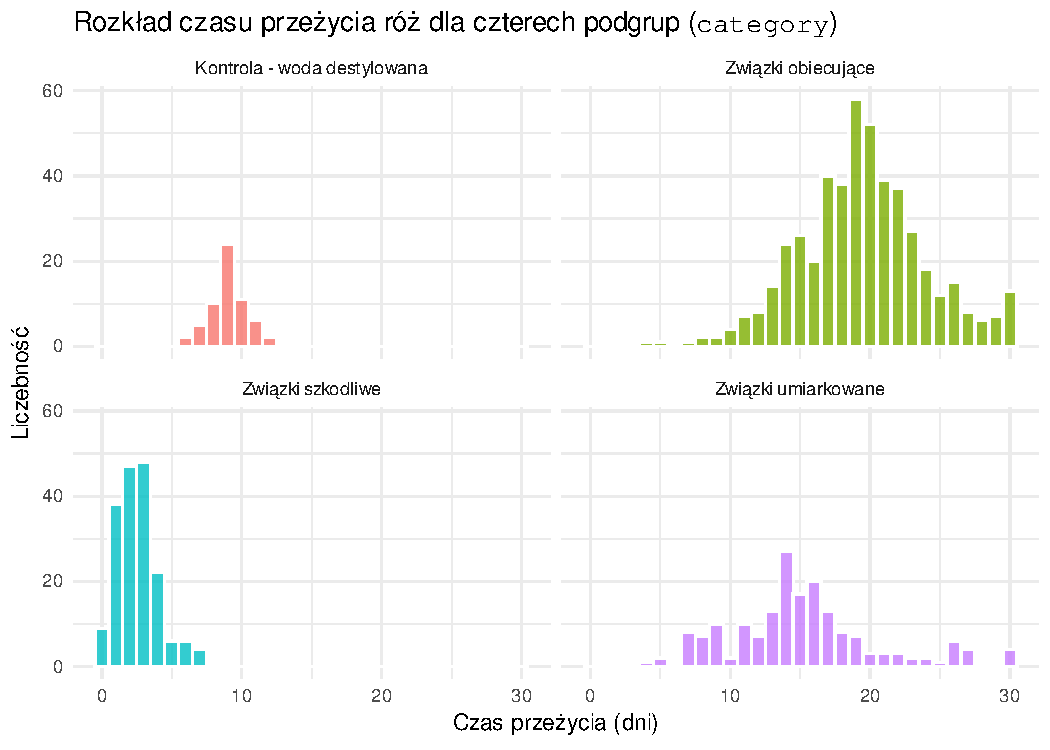
\includegraphics[width=0.85\textwidth]{plots/group_surv_time_hist.pdf}
    \caption{Rozkłady zmiennej \texttt{time} dla czterech grup związków -- \texttt{category}.}
    \label{fig:surv_time_hist_comp}
\end{figure}

\par Rozkłady czasu przeżycia dla poszczególnych grup przedstawiono na Rycinie~\ref{fig:surv_time_hist_comp}. Wizualizacja potwierdza istotne zróżnicowanie pomiędzy grupami oraz pozwala jednoznacznie wskazać silny wpływ zarówno związków szkodliwych, jak i związków obiecujących na obserwowaną dwumodalność rozkładu zmiennej \texttt{time}. W grupie związków szkodliwych dominują krótkie czasy przeżycia, co wskazuje na wysoką toksyczność i szybkie obumieranie kwiatów. Z kolei w grupie związków obiecujących obserwuje się przesunięcie rozkładu w stronę dłuższych czasów przeżycia, co świadczy o pozytywnym wpływie zastosowanych substancji na trwałość róż.

% ============================================================
% ROZKŁAD PRZEŻYCIA WEDŁUG ZASTOSOWANEGO ZWIĄZKU
% ============================================================
\subsection{Rozkład przeżycia kwiatów według zastosowanego związku}\label{subsec:compounds_distributon}

\par W celu oceny zróżnicowania czasu przeżycia róż w zależności od zastosowanego związku sporządzono wykres typu ramka–wąsy, przedstawiony na Rycinie~\ref{fig:compounds_boxplot}. Wizualizacja ta umożliwia porównanie median, rozstępów międzykwartylowych oraz obecności obserwacji odstających pomiędzy poszczególnymi substancjami, co pozwala na wstępną ocenę ich wpływu na zmienną \texttt{time}.

% 2. boxplot czasu przeżycia według compound (szczegółowy rozkład per substancja)
\begin{figure}[h!]
    \centering
    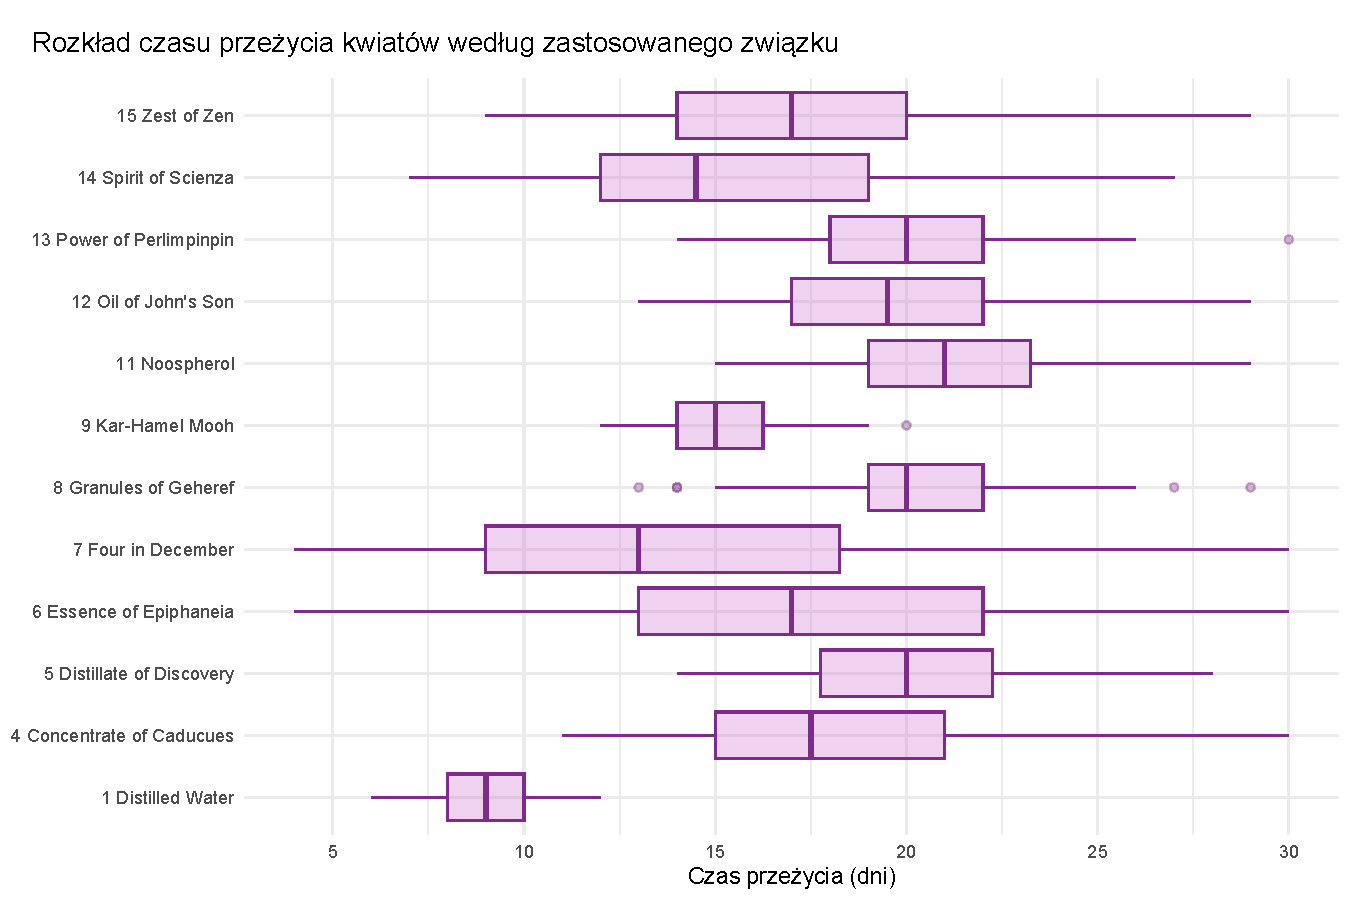
\includegraphics[width=1\textwidth]{plots/boxplot_compounds.pdf}
    \caption{Rozkład zmiennej \texttt{time} według zastosowanego związku.}
    \label{fig:compounds_boxplot}
\end{figure}

\par Wizualne porównanie rozkładów czasu przeżycia kwiatów sugeruje niewielką zmienność dla związków należących do grupy \textcolor{TealBlue}{szkodliwej} (2, 3 i 10). Przedziały międzykwartylowe (IQR) rozkładów tych roztworów są wąskie (maksymalna długość przedziału w tej grupie wynosi zaledwie 2). W kontekście biologicznym oznacza to, że kwiaty zanurzone w tych substancjach przeżywały zaledwie kilka dni oraz ich obserwowane czasy przeżycia były do siebie bardzo zbliżone. Związki te charakteryzują się \textbf{stabilnie niekorzystnym} działaniem na wydłużenie czasu przeżycia róż. 

\par Grupa \textcolor{Orchid}{umiarkowana} (7, 9 i 14) charakteryzuje się znacznie większym zróżnicowaniem wewnętrznym. Najstabilniejsze działanie wykazuje związek 9, dla którego rozstęp międzykwartylowy (IQR) wynosi zaledwie 2,2 dnia. W przeciwieństwie do niego, związki 7 i 14 cechują się znacznie większą zmiennością, IQR odpowiednio 9,2 i 7, co sugeruje mniejszą przewidywalność ich wpływu na trwałość kwiatów.

\par Grupa \textcolor{YellowGreen}{obiecująca} obejmuje zarówno związki o dużej zmienności (4, 6, 15), jak i te o umiarkowanym oraz małym zróżnicowaniu wyników (5, 8, 11, 12, 13). Sugeruje to, że mimo ogólnie korzystnego działania na wydłużenie czasu przeżycia róż, skuteczność poszczególnych związków różni się pod względem stabilności działania.

\par \textcolor{Salmon}{Grupa kontrolna} -- woda destylowana, stanowi jeden z najstabilniejszych związków z rozstępem międzykwartylowym wynoszącym 2, medianą dziewięciu dni oraz brakiem obserwacji odstających.

\par Wartości odstające, które w znacznym stopniu odbiegają od typowych wyników w danej grupie, odnotowano dla następujących związków: 8, 9, 10 oraz 13. W przypadku toksycznego związku \textit{Lucifer's Liquid}, wystąpienie obserwacji wykraczającej poza zakres górnego wąsa sugerować może okaz cechujący się wyższą tolerancją na szkodliwy czynnik. Dla pozostałych związków, tj. 8, 9 oraz 13, wartości odstające występują głównie powyżej górnego wąsa, co wskazuje na pojedyncze obserwacje o wyraźnie dłuższym czasie przeżycia. Może to świadczyć o indywidualnych różnicach w reakcji badanych kwiatów na zastosowane roztwory. W przypadku związku 8 zaobserwowano również niższe wartości odstające, co dodatkowo podkreśla większą niejednorodność odpowiedzi oraz zróżnicowaną skuteczność działania tej substancji. Formalne porównanie funkcji przeżycia dla poszczególnych związków przedstawiono w kolejnej części.

% ============================================================
% KRZYWE PRZEŻYCIA WEDŁUG ZASTOSOWANEGO ZWIĄZKU
% ============================================================
\subsection{Krzywe przeżycia według zastosowanego związku}\label{subsec:km_compounds}

W celu dokładniejszej eksploracji działania badanych związków na trwałość róż przygotowano Rycinę~\ref{fig:compounds_km} krzywych przeżycia Kaplana-Meiera. Każdy z piętnastu paneli przedstawia krzywą oraz przedział ufności dla danego związku wraz z zaznaczoną szarym kolorem krzywą odnoszącą się do grupy kontrolnej -- wody destylowanej. Krzywa przeżycia dla grupy \textcolor{Salmon}{kontrolnej} cechuje się stosunkowo stromym nachyleniem oraz wąskim przedziałem ufności. 

\begin{figure}[h!]
    \centering
    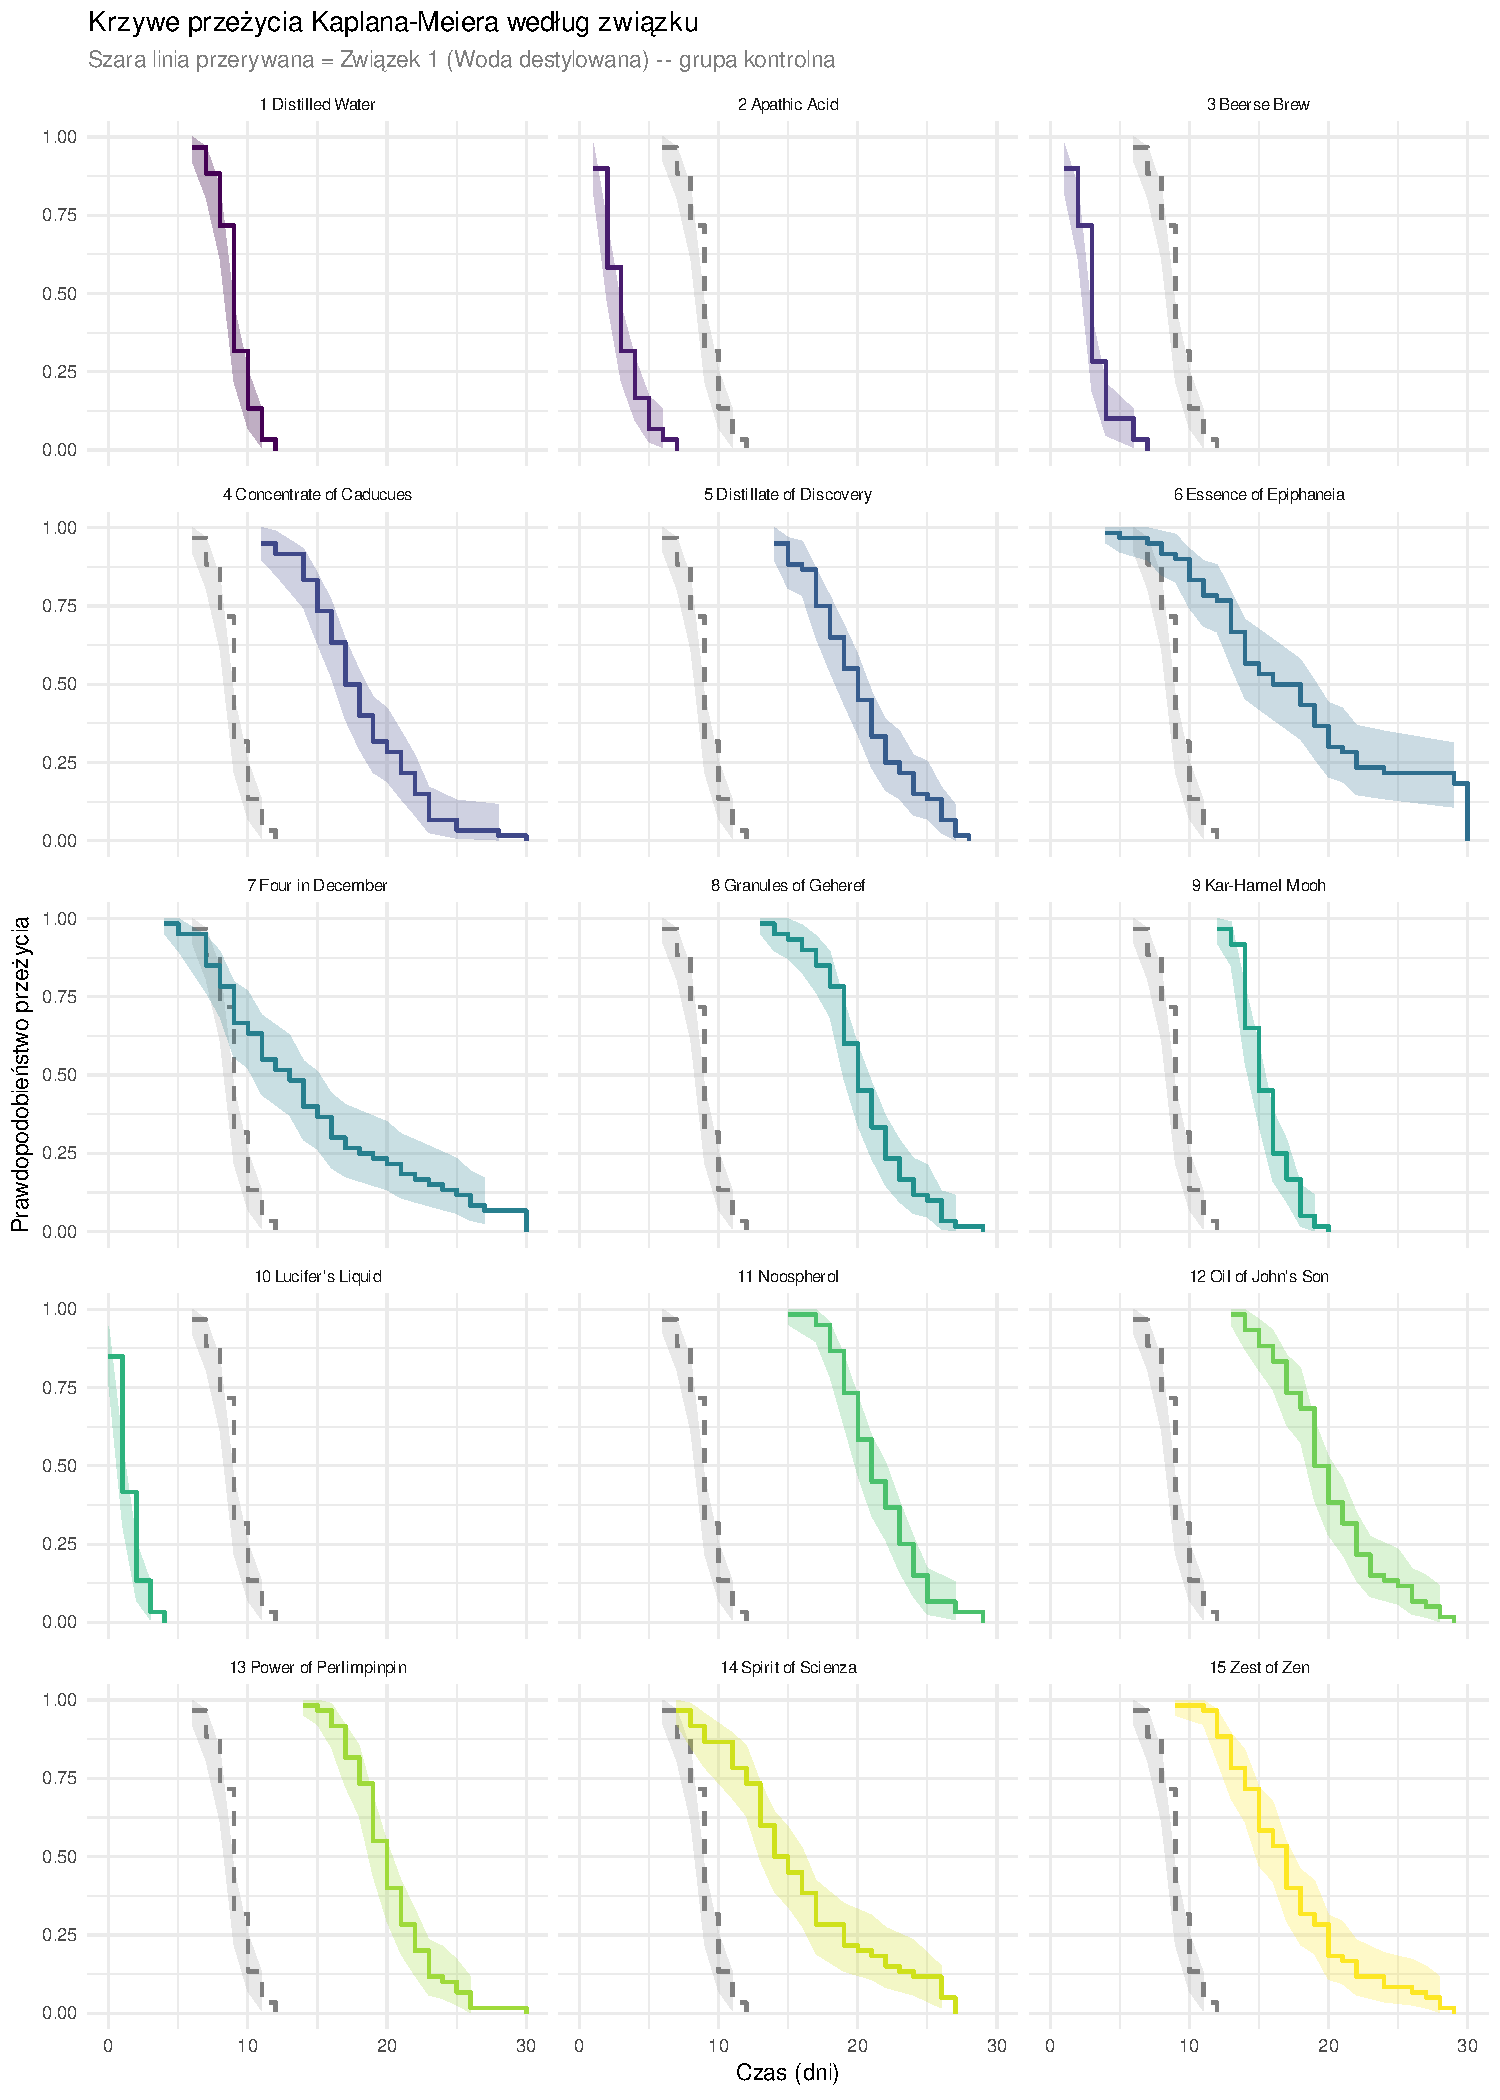
\includegraphics[width=1\textwidth, height = 18cm]{plots/km_compounds_facet.pdf}
    \caption{Krzywe przeżycia Kaplana-Meiera według zastosowanego związku.}
    \label{fig:compounds_km}
\end{figure}

\par Krzywe Kaplana-Meiera dla związków \textcolor{TealBlue}{szkodliwych} (2, 3, 10) przebiegają znacznie poniżej poziomu kontrolnego. Cechują się gwałtownym spadkiem prawdopodobieństwa przeżycia już od momentu rozpoczęcia eksperymentu. Ich strome nachylenie oraz wąskie przedziały ufności sugerują wysoką toksyczność roztworów oraz niemal jednoczesne obumieranie większości kwiatów w tych grupach.

\par Związki należące do grupy \textcolor{Orchid}{umiarkowanej} (7, 9, 14) charakteryzują się przebiegiem krzywych zbliżonych do grupy kontrolnej. Krzywe znajdują się blisko grupy kontrolnej, pokrywając się, bądź zachowując zbliżony kształt, co wskazuje na podobny wzorzec przeżycia i umiarkowane działanie związków na przeżywalność kwiatów.

\par Najliczniejsza grupa związków \textcolor{YellowGreen}{obiecujących} cechuje się przebiegiem krzywych powyżej krzywej kontrolnej, wskazując na wydłużony czas przeżycia kwiatów. Szczególnie wyraźne odchylenie od grupy kontrolnej obserwowane jest dla związków: 8, 11, 13, w przypadku, których prawdopodobieństwo przeżycia po upływie 20 dni nadal wynosiło około 50\%. Dla części związków przedziały ufności w niewielkim stopniu nakładają się na przedział grupy kontrolnej (6, 14).

\par Zdecydowana większość krzywych wykazuje płynny, monotoniczny spadek i wskazuje na stopniowe narastanie ryzyka w czasie. Wykres ten ma charakter wyłącznie eksploracyjny, stanowi podstawę do zastosowania modelu Weibulla oraz uzasadnia wykorzystanie zmiennej \texttt{compound} jako zmiennej wyjaśniającej, kategorycznej w tymże modelu.

% ============================================================
% KRZYWE PRZEŻYCIA DLA ZMIENNYCH: GARDEN I SPECIES
% ============================================================
\subsection{Krzywe przeżycia według zmiennych \texttt{garden} i \texttt{species}}\label{subsec:km_garden_species}
Krzywe przeżycia Kaplana-Meiera według ogrodu, z którego pochodziły jednostki eksperymentalne przedstawiono na Rycinie~\ref{fig:garden_km}, natomiast analogiczny wykres według gatunku róż na Rycinie~\ref{fig:species_km}.
% Krzywa KM - ogród
\begin{figure}[h!]
    \centering
    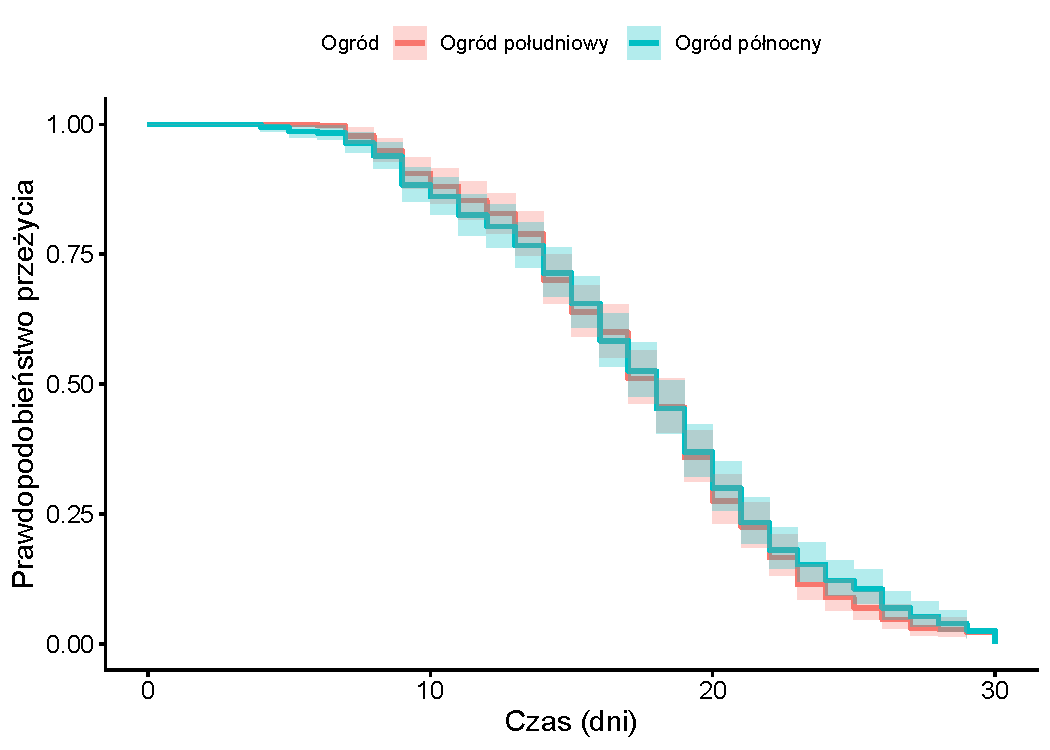
\includegraphics[width=0.8\textwidth]{plots/garden_km.pdf}
    \caption{Krzywa przeżycia Kaplana-Meiera według ogrodu.}
    \label{fig:garden_km}
\end{figure}
% Krzywa KM - gatunek

\begin{figure}[h!]
    \centering
    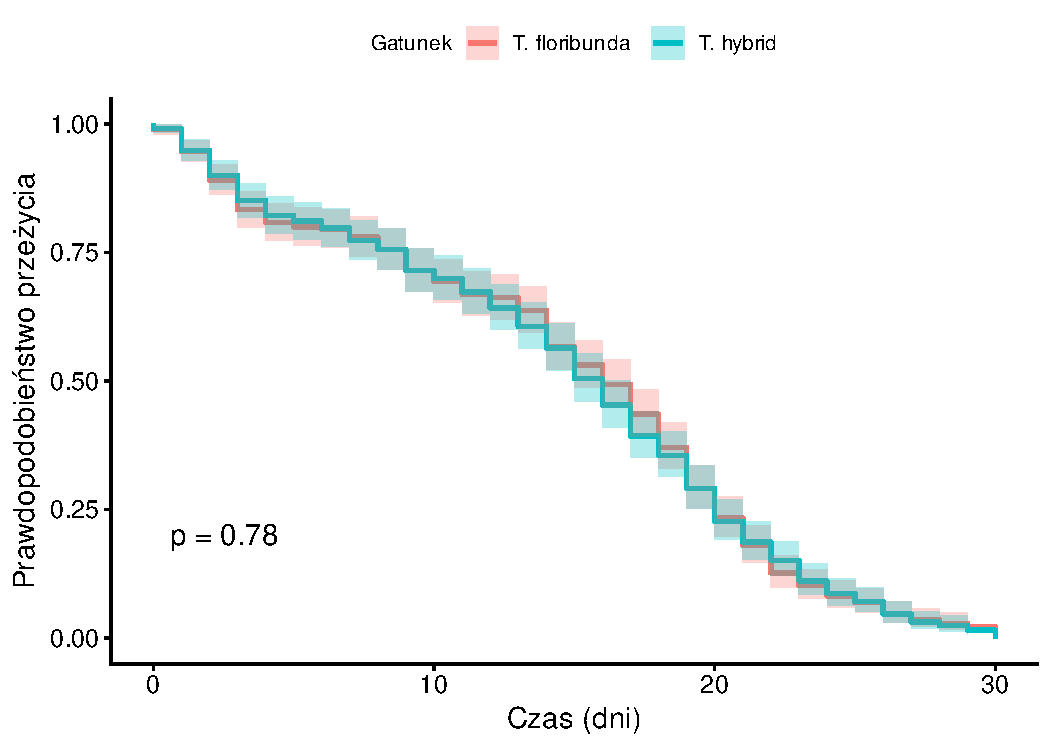
\includegraphics[width=0.8\textwidth]{plots/species_km.pdf}
    \caption{Krzywa przeżycia Kaplana-Meiera według gatunku róży.}
    \label{fig:species_km}
\end{figure}

W obu przypadkach nie stwierdzono istotnych różnic w przeżywalności między grupami. Test log-rank nie wykazał istotnych statystycznie różnic dla ogrodu (p-value = 0,55) ani dla gatunku (p = 0,78), a krzywe niemal całkowicie się pokrywały. Krzywe w obu przypadkach nie przecinają się, co potwierdza zasadność założenia proporcjonalnych hazardów dla obu zmiennych.

% ============================================================
% OCENA ZASADNOŚCI MODELU WEIBULLA - CLOGCLOG
% ============================================================
\subsection{Ocena zasadności modelu Weibulla}\label{subsec:cloglog}
W celu oceny zasadności zastosowania modelu Weibulla sporządzono wykres~\ref{fig:cloglog} \textbf{CLogLog}: $\log(-\log \hat{S}(t))$ w funkcji $\log(t)$ (ang. \textit{Complementary log-log}) dla czterech grup związków. 

\begin{figure}[h!]
    \centering
    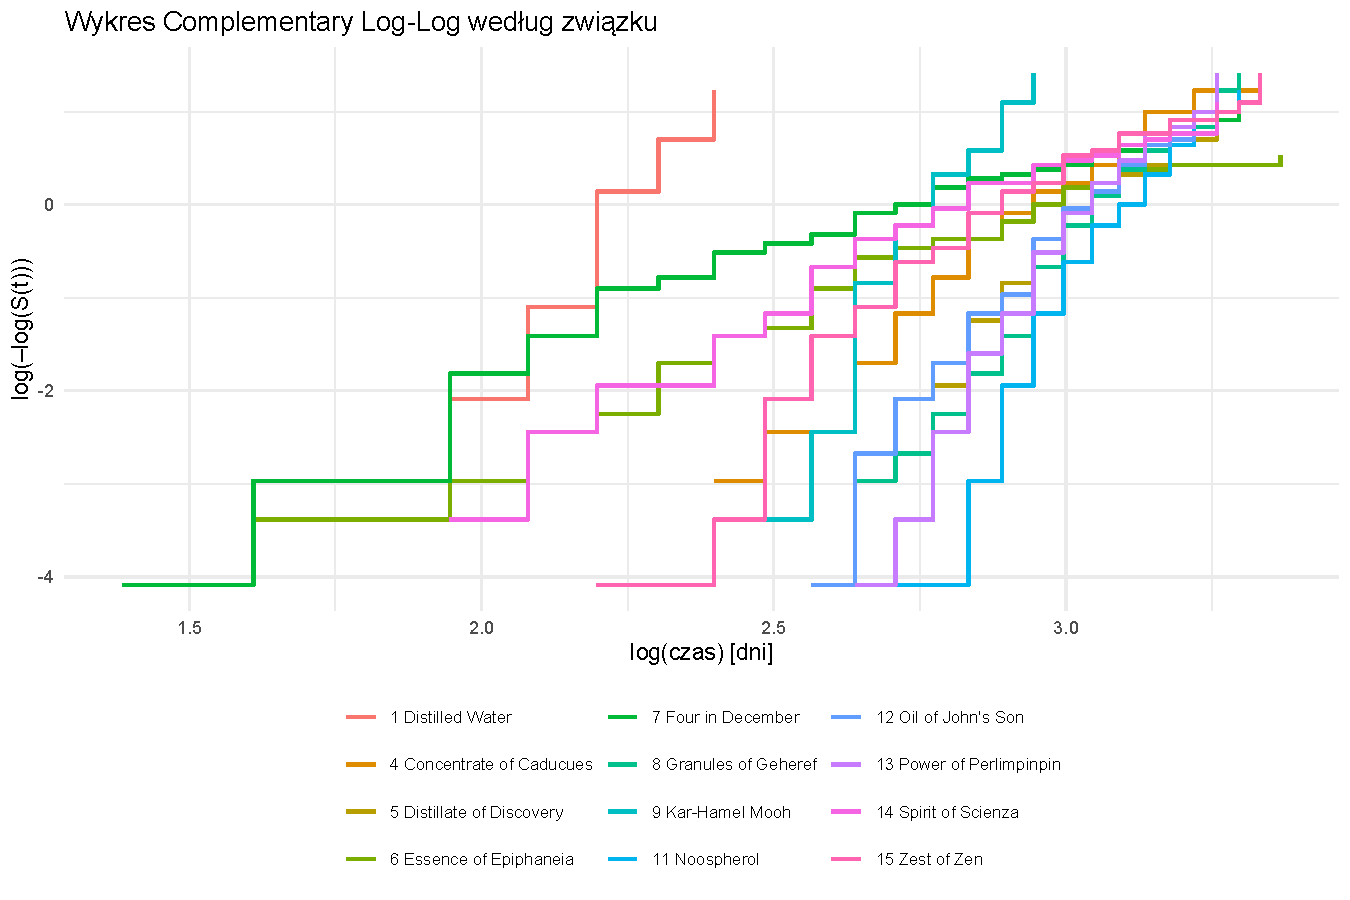
\includegraphics[width=0.8\textwidth]{plots/cloglog.pdf}
    \caption{Wykres CLogLog dla czterech grup związków.}
    \label{fig:cloglog}
\end{figure}

\par W przypadku grup uwzględnionych w analizie głównej (kontrolna, umiarkowana, obiecująca) obserwowane krzywe wykazują liniowość oraz przebiegają w przybliżeniu równolegle, co uzasadnia wykorzystanie modelu Weibulla z proporcjonalnymi hazardami i wspólnym parametrem kształtu $k$. 
\par Grupa związków szkodliwych odbiega od tego założenia, cechując się wyraźnymi odchyleniami od liniowości, spowodowanymi silną koncentracją występowania zdarzeń w pierwszych dniach eksperymentu. Z tego względu obserwacje należące do omawianej grupy zostały wyłączone z analizy głównej. 
\par W wyniku dopasowania modelu Weibulla metodą największej wiarygodności do danych pilotażowych (z wyłączeniem związków szkodliwych) uzyskano estymację parametru kształtu $\hat{k} = 4{,}36$. Wynik ten potwierdza tendencję wzrostową hazardu wraz z upływem czasu ($k > 1$) zgodną z biologicznym procesem pogarszania się kondycji kwiatów w czasie. Uzyskaną wartość wykorzystano do kalibracji rozkładu a priori parametru kształtu w modelu bayesowskim. W tym samym modelu oceniono również wpływ zmiennej \texttt{baseline\_diam} na czas przeżycia. Współczynnik w modelu był nieistotny statystycznie ($p = 0{,}574$), co stanowiło podstawę do wykluczenia tej zmiennej z modelu głównego.

% ============================================================
\section{Specyfikacja modelu statystycznego}\label{sec:model_structure}
% ============================================================
Analiza główna przeprowadzona zostanie w paradygmacie bayesowskim, w którym wnioskowanie o parametrach modelu oparte jest na rozkładzie a posteriori:

\begin{equation}
    posterior \propto likelihood \cdot prior
    \label{eq:posterior}
\end{equation}

Rozkład a posteriori łączy zatem informację zawartą w danych z wiedzą a priori badacza o parametrach modelu.
\subsection{Model przeżycia Weibulla}\label{subsec:weibull_model}

Główną część analizy statystycznej stanowi parametryczny model przeżycia oparty na rozkładzie Weibulla. Rozkład ten znajduje szerokie zastosowanie w modelowaniu procesów biologicznych, charakteryzujących się narastającym hazardem w czasie. W przypadku kwiatów będących przedmiotem tej analizy, obserwuje się intensyfikację procesu utraty świeżości oraz obumieranie rośliny wraz z upływem czasu, co idealnie wpisuje się we wspomnianą wcześniej specyfikę rozkładu Weibulla. W wyniku weryfikacji warunku koniecznego dla zastosowania rozkładu Weibulla w sekcji~\ref{subsec:cloglog} na podstawie danych pilotażowych, potwierdzono liniowość krzywych $\log(-\log\hat{S}(t))$ względem $\log(t)$ dla grup uwzględnionych w głównej analizie.

Założono, że dla każdej $i$-tej róży czas przeżycia $T_i$ ma następujący rozkład oraz funkcję przeżycia, która określa prawdopodobieństwo, że dana jednostka przeżyje dłużej niż dany czas $t$:

\begin{equation}
    T_i \sim \mathrm{Weibull}(k,\, \lambda_i), \qquad
    S(t \mid k, \lambda_i) = \exp\!\left[-\!\left(\frac{t}{\lambda_i}\right)^{\!k}\right]
    \label{eq:weibull_model}
\end{equation}

gdzie $k > 0$ jest wspólnym parametrem kształtu, a $\lambda_i > 0$ jest parametrem skali  jednostki $i$. Parametr skali $\lambda_i$ zależy od zmiennych objaśniających i jest modelowany na skali logarytmicznej:

\begin{equation}
    \log \lambda_i = \beta_0 + \alpha_{c(i)} + \gamma_{s(i)} + b_{g(i)}
    \label{eq:linear_predictor}
\end{equation}

gdzie:
\begin{itemize}[noitemsep]
    \item $\beta_0$ -- wyraz wolny; logarytm parametru skali grupy kontrolnej (związek 1), gatunku referencyjnego (\textit{T. floribunda}) oraz przeciętnego efektu ogrodu,
    \item $\alpha_{c(i)}$ -- efekt stały związku $c(i)$; $c(i) \in \{1, 4, 5, 6, 7, 8, 9, 11, 12, 13, 14, 15\}$, przyjmując związek 1 (woda destylowana) jako grupę referencyjną, dla której $\alpha_1 = 0$,
    \item $\gamma_{s(i)}$ -- efekt stały gatunku róży $s(i) \in \{1, 2\}$, przyjmując gatunek \textit{T. floribunda} (species 1) jako grupę referencyjną, dla której $\gamma_1 = 0$ ,
    \item $b_{g(i)} \sim \mathcal{N}(0,\, \sigma_g^2)$ -- efekt losowy ogrodu $g(i) \in \{1, 2\}$.
\end{itemize}

Obserwacje prawostronnie cenzurowane uwzględniane są w funkcji 
wiarygodności zgodnie ze standardowym podejściem analizy przeżycia.
Niech $\delta_i$ oznacza wskaźnik wystąpienia zdarzenia dla $i$-tej jednostki:

\begin{equation}
    \delta_i = \begin{cases}
        1 & \text{jeśli zdarzenie wystąpiło (róża obumarła),} \\
        0 & \text{jeśli obserwacja jest cenzurowana.}
    \end{cases}
\end{equation}

Wówczas funkcja wiarygodności dla wszystkich $n$ jednostek przyjmuje następującą postać \parencite{qian1994}:

\begin{equation}
    L(\mathbf{t} \mid k, \boldsymbol{\lambda}) = 
    \prod_{i=1}^{n} f(t_i \mid k, \lambda_i)^{\delta_i} \cdot 
    S(t_i \mid k, \lambda_i)^{1-\delta_i}
    \label{eq:likelihood}
\end{equation}

\begin{equation}\label{eq:weibull_density}
    f(t_i \mid k, \lambda_i) = \frac{k}{\lambda_i}\!\left(\frac{t_i}{\lambda_i}\right)^{k-1}
    \exp\!\left[-\!\left(\frac{t_i}{\lambda_i}\right)^k\right]
\end{equation}

gdzie $f(t_i \mid k, \lambda_i)$ (równanie~\eqref{eq:weibull_density}) jest funkcją gęstości rozkładu Weibulla, a $S(t_i \mid k, \lambda_i)$ 
(równanie~\eqref{eq:weibull_model}) jest funkcją przeżycia. Jednostki, dla których wystąpiło zdarzenie 
($\delta_i = 1$), wnoszą do wiarygodności pełną gęstość $f(t_i)$, z kolei 
jednostki prawostronnie cenzurowane ($\delta_i = 0$) wyłącznie $S(t_i)$, co odzwierciedla jedynie fakt przeżycia do czasu $t_i$.
W przypadku danych pilotażowych odsetek obserwacji cenzurowanych wyniósł 0\%, 
zatem wszystkie jednostki wnoszą pełną gęstość do funkcji wiarygodności.


\par\textbf{Interpretacja parametrów}: 
\par Parametr kształtu $k$ określa charakter funkcji hazardu $h(t) = (k/\lambda)(t/\lambda)^{k-1}$, gdzie:
\begin{itemize}
    \item $k > 1$ -- narastający hazard (ryzyko obumarcia rośnie wraz z czasem)
    \item $k = 1$ -- stały hazard (ryzyko obumarcia jest stałe w czasie,
    Weibull($k=1$, $\lambda$) = Exp($\lambda$))
    \item  $k < 1$ -- malejący hazard (ryzyko obumarcia maleje wraz z czasem)
\end{itemize} Na podstawie danych pilotażowych uzyskano estymowaną wartość parametru $\hat{k} = 4{,}36$, co potwierdza narastający charakter hazardu w procesie starzenia się kwiatów. 
\par Efekty związków $\alpha_c$ interpretowane są jako logarytm ilorazu czasów przeżycia: $\exp(\alpha_c)$ oznacza czynnik, o jaki zmienia się czas przeżycia kwiatu pod wpływem związku $c$ w porównaniu z grupą kontrolną (wodą destylowaną). Wartość $\alpha_c > 0$ świadczy o wydłużonym czasie przeżycia (działanie korzystne), a $\alpha_c < 0$ -- o skróconym (działanie szkodliwe). 
\par Analogicznie, efekt gatunku $\gamma_s$ interpretowany jest jako logarytm ilorazu czasów przeżycia między gatunkami: $\exp(\gamma_s)$ oznacza czynnik, o jaki różni się czas przeżycia gatunku 2 (\textit{T. hybrid}) względem gatunku referencyjnego (\textit{T. floribunda}), przyjmując ten sam związek i ogród.

\subsection{Zmienne objaśniające i uzasadnienie ich doboru}

Na podstawie eksploracyjnej analizy danych pilotażowych oraz wyników dopasowania do nich modelu Weibulla podjęto następujące decyzje dotyczące doboru zmiennych do ostatecznego modelu:

\begin{itemize}
    \item \textbf{Związek (\texttt{compound})} -- uwzględniony jako kategoryczna zmienna stała. Punkt odniesienia stanowi związek 1 -- woda destylowana, w modelu odpowiednio $\alpha_1 = 0$. Zmienna ta stanowi główny przedmiot zainteresowania analizy.

    \item \textbf{Ogród (\texttt{garden})} -- uwzględniony jako efekt losowy ($b_g \sim \mathcal{N}(0, \sigma_g^2)$), pomimo braku istotnych różnic w przeżywalności między ogrodami na podstawie danych pilotażowych (log-rank: $p = 0{,}55$). Wprowadzenie zmiennej blokującej ogród miało na celu kontrolę potencjalnej zmienności środowiskowej jednostek eksperymentalnych i stanowiło jedno z założeń schematu badania, dlatego bez względu na nieistotne wyniki testu log-rank włączono ją do modelu. Ogród uwzględniono jako efekt losowy, ponieważ dwa ogrody objęte badaniem stanowią próbę z szerszej populacji możliwych warunków uprawy, a celem analizy jest uogólnienie wniosków poza te konkretne lokalizacje.

    \item \textbf{Gatunek (\texttt{species})} -- uwzględniony jako efekt stały w modelu. Podobnie jak w przypadku zmiennej \texttt{garden}, w analizie eksploracyjnej danych pilotażowych nie wykryto istotnych różnic w przeżywalności między gatunkami róż (log-rank: $p = 0{,}78$). Analogicznie ze względu na przyjęty schemat eksperymentu zmienna gatunek stanowi część modelu. Gatunek uwzględniono jako efekt stały, ponieważ przedmiotem zainteresowania jest konkretna różnica między dwoma badanymi gatunkami.

    \item \textbf{Średnica kwiatostanu (\texttt{baseline\_diam})} -- wykluczona z analizy głównej. Współczynnik dla tej zmiennej w modelu Weibulla dopasowanym do danych pilotażowych z uwzględnieniem \texttt{compound} był bliski zeru i nieistotny statystycznie ($p = 0{,}574$ Sekcja~\ref{subsec:cloglog}).

    \item \textbf{Związki szkodliwe (2, 3, 10)} -- wykluczone z analizy głównej. Na podstawie analizy eksploracyjnej danych pilotażowych stwierdzono, że substancje te powodują gwałtowne obumieranie kwiatów (mediana przeżycia 1--3 dni, znacznie poniżej grupy kontrolnej, dla której mediana wynosiła 9 dni) i wykazują wyraźne odchylenia od założenia proporcjonalnych hazardów (Rycina~\ref{fig:cloglog}). Głównym celem analizy jest natomiast identyfikacja związków potencjalnie wydłużających czas przeżycia kwiatów względem przyjętej grupy kontrolnej, zatem wymienione związki nie będą częścią głównego eksperymentu oraz analizy.
\end{itemize}

\subsection{Rozkłady a priori}\label{subsec:priors}
Podejście bayesowskie zakłada, że każdy nieznany występujący w modelu parametr opisany jest własnym rozkładem a priori. Rozkład ten odzwierciedla aktualny stan wiedzy badacza o danym predyktorze w modelu. W zależności od posiadanej wiedzy możliwe jest zastosowanie rozkładów nieinformacyjnych/słabo informacyjnych, które stanowią stosunkowo,,liberalne'' podejście, nie narzucając silnych założeń dotyczących wartości parametru, bądź przyjęcie rozkładów informacyjnych (podejście bardziej ,,konserwatywne''), poprzedzonych na przykład wynikami wcześniejszych podobnych badań lub wiedzą ekspercką. W przypadku niniejszej analizy rozkłady a priori parametrów modelu Weibulla wyznaczono na podstawie wyników analizy pilotażowej oraz prior predictive check, działania polegającego na generowaniu danych z rozkładów a priori i ocenie, czy otrzymane krzywe przeżycia są biologicznie wiarygodne. Dane pilotażowe wykorzystane zostały wyłącznie w celu kalibracji rozkładów a priori i nie były uwzględniane w estymacji głównego modelu. Podejście to pozwoliło na uniknięcie nadmiernego zawężenia rozkładów a priori, którego przyczyną mogłoby być ponowne wykorzystanie tych samych informacji (ang. \textit{double-counting}).

\subsubsection{Parametr kształtu $k$}

\begin{equation}
    k \sim \mathrm{Gamma}(15{,}466;\; 3{,}544), \qquad \mathbb{E}[k] = 4{,}363, \quad \mathrm{SD}(k) \approx 1{,}11, \quad \mathrm{P}(k > 1) \approx 99{,}99\%
    \label{eq:prior_k}
\end{equation}

Wybór rozkładu Gamma jako kandydata na rozkład a priori parametru $k$ w naturalny sposób gwarantuje spełnienie warunku wynikającego z założeń rozkładu Weibulla, dla którego parametr kształtu $k \in \left(0, +\infty\right)$. Parametry $\alpha$ oraz $\beta$ wyznaczono w dwóch etapach:

\begin{enumerate}
    \item \textbf{Kalibracja parametrów rozkładu na podstawie danych pilotażowych.} \\
    Globalne dopasowanie wspólnego modelu Weibulla z efektem związku (\texttt{compound}) jako predyktorem, metodą największej wiarygodności do danych pilotażowych (z wyłączeniem związków szkodliwych -- omówione w Sekcji~\ref{subsec:cloglog}). Oszacowane odchylenie standardowe zostało powiększone dwukrotnie, aby zapobiec przyjęciu zbyt wąskiego rozkładu a priori. Parametry rozkładu Gamma wyznaczono wykorzystując metodę momentów, gdzie $\alpha = \frac{E[X]^2}{V[X]}, \beta = \frac{E[X]}{V[X]}$, stąd dla wartości oczekiwanej $E[k] \approx 4{,}363$ oraz wariancji $V[k] \approx 1{,}231$ otrzymano odpowiednio $\alpha \approx 15{,}466$ oraz $\beta \approx 3{,}544$.

    \item \textbf{Prior predictive check.} \\
    Zasadność przyjętego rozkładu a priori zweryfikowano, próbkując 300 wartości $k$ z rozkładu $\mathrm{Gamma}(15{,}466;\; 3{,}544)$ i generując odpowiadające im krzywe przeżycia Weibulla przy $\lambda$ skalibrowanym do mediany grupy kontrolnej wynoszącej 9 dni (Rycina~\ref{fig:prior_pred_surv}). Wszystkie wygenerowane krzywe przeżycia wykazywały biologicznie wiarygodny przebieg procesu obumierania kwiatów. 
\end{enumerate}

Przyjęty rozkład a priori przypisuje prawdopodobieństwo $P(k > 1) \approx 99{,}99\%$, silnie faworyzując narastający hazard zgodny z biologicznym procesem starzenia kwiatów, a jednocześnie zapewnia wystarczające rozproszenie (95\% przedział a priori: $[2{,}47;\; 6{,}79]$), by nie zatracić informacji z danych głównych. Graficzną ilustrację rozkładu a priori wraz z oznaczoną estymacją pilotażową oraz wyniki prior predictive check przedstawiono na Rycinach~\ref{fig:prior_k_density} i~\ref{fig:prior_pred_surv}.

\begin{figure}[h!]
    \centering
        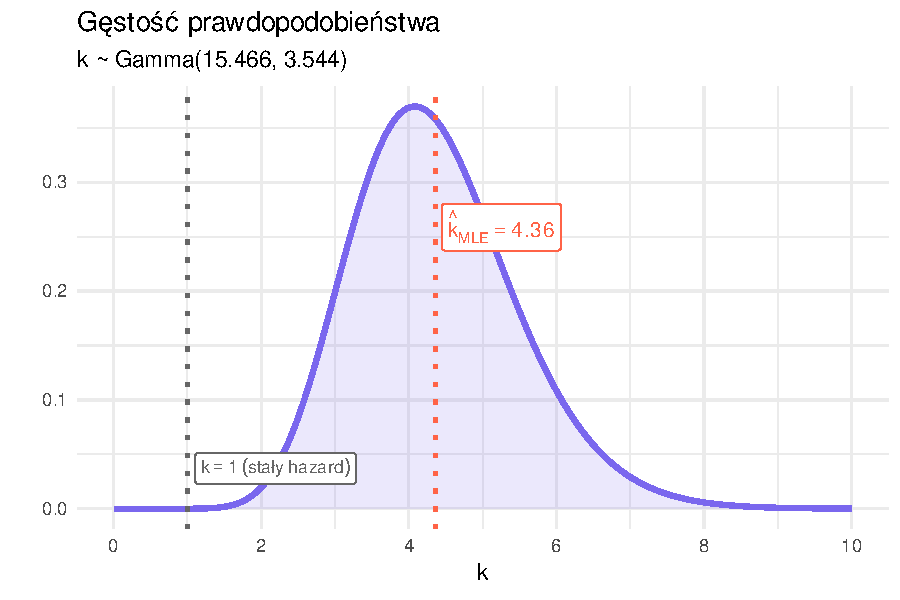
\includegraphics[width=0.8\textwidth]{plots/prior_k_density.pdf}
        \caption{Rozkład a priori parametru kształtu $k$. Czerwona linia przerywana: $\hat{k}_{\mathrm{MLE}} = 4{,}36$ z danych pilotażowych.}
        \label{fig:prior_k_density}
\end{figure}
\begin{figure}[h!]
        \centering
        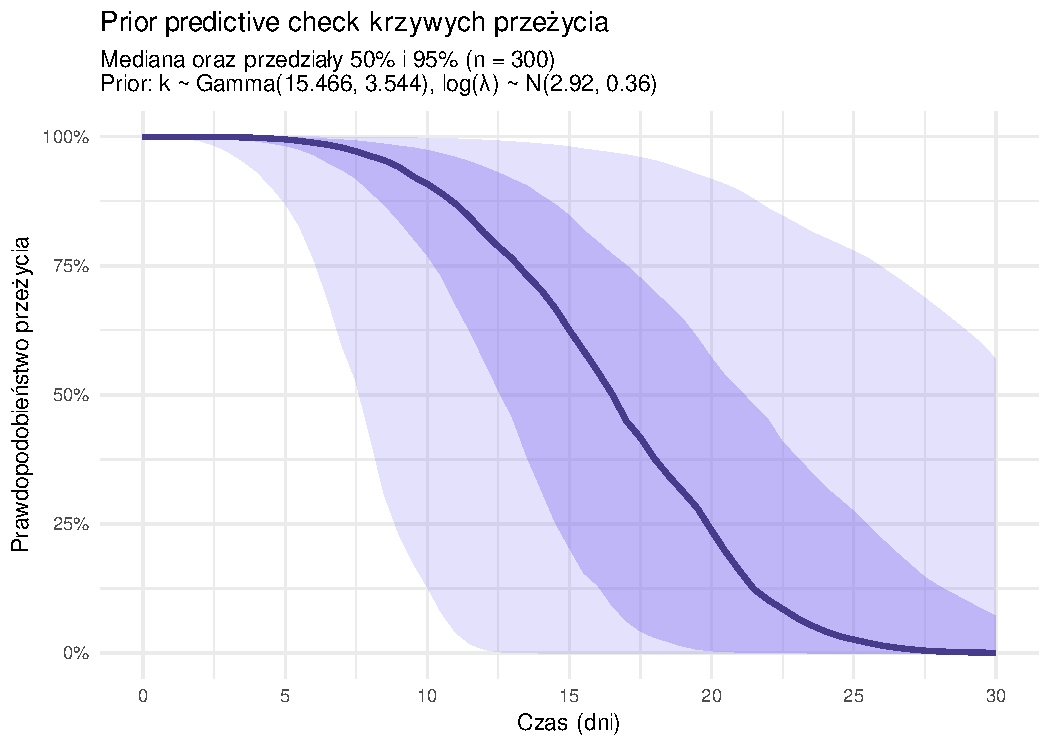
\includegraphics[width=0.8\textwidth]{plots/prior_pred_surv.pdf}
        \caption{Prior predictive check: 300 krzywych przeżycia wygenerowanych z $k \sim \mathrm{Gamma}(15{,}466;\; 3{,}544)$.}
        \label{fig:prior_pred_surv}
\end{figure}
\newpage
\subsubsection{Parametry skali: wyraz wolny $\beta_0$ i efekty $\alpha_c$, $\gamma_s$ (skala $\log\lambda$)}

\begin{align}
    \beta_0 &\sim \mathcal{N}(2{,}918; 0{,}363) \\
    \alpha_c &\sim \mathcal{N}(0; 0{,}22) \\
    \gamma_s &\sim \mathcal{N}(0; 0{,}22)
\end{align}

\par Wartość oczekiwaną $E[\beta_0] = 2{,}918$ rozkładu a priori parametru $\beta_0$ otrzymano w wyniku dopasowania modelu Weibulla zawierającego wyłącznie wyraz wolny do każdej z możliwych unikalnych kombinacji czynników \texttt{compound} $\times$ \texttt{species} $\times$ \texttt{garden} w danych pilotażowych. Dla każdej z grup wyestymowano parametr $\log(\hat{\mu})$, który odnosi się do typowego logarytmu czasu przeżycia w danej grupie. Ostatecznie uśredniając otrzymane estymacje otrzymano wartość oczekiwaną rozkładu a priori parametru $\beta_0$. Wartość odchylenia standardowego dla otrzymanych estymacji powiększono 1,5 razy, aby nie otrzymać nazbyt wąskiego rozkładu a priori, stąd ostateczna wartość odchylenia standardowego wyniosła 0{,}363.

\par W przypadku parametrów $\alpha_c$ oraz $\gamma_s$ za wartość oczekiwaną przyjęto 0, nie zakładając uprzednio, że czynniki te wpływają na wydłużenie, bądź skrócenie czasu przeżycia kwiatów. Otrzymane wcześniej (przy estymacji parametrów rozkładu a priori $\beta_0$) wartości $\log(\hat{\mu})$ wykorzystano w celu wyznaczenia odchylenia standardowego. Pogrupowanie komórek względem \texttt{compound} $\times$ \texttt{species} oraz uśrednienie wartości $\log(\hat{\mu})$ w obrębie każdej grupy po ogrodach, pozwoliło wyeliminować zmienność wynikającą z ogrodu. Odchylenie standardowe obliczone na podstawie tak otrzymanych średnich grupowych wyniosło $0{,}22$ i zostało przyjęte jako parametr rozkładów a priori dla $\alpha_c$ oraz $\gamma_s$. Wartości odchylenia standardowego nie powiększano, gdyż odzwierciedla ono rzeczywiste zróżnicowanie między grupami w danych pilotażowych. Ten sam rozkład a priori przyjęto dla $\alpha_c$ oraz $\gamma_s$, gdyż oba parametry działają na tej samej skali $\log\lambda$, a przyjęcie wspólnego rozkładu stanowi swego rodzaju uproszczenie uzasadnione ograniczoną liczebnością danych pilotażowych.

\subsubsection{Odchylenie standardowe efektu losowego ogrodu $\sigma_g$}

\begin{equation}
    \sigma_g \sim \mathrm{HalfNormal}(0;\ 0{,}283)
    \label{eq:prior_sigma_g}
\end{equation}

Rozkład półnormalny gwarantuje dodatniość parametru $\sigma_g$, który jako odchylenie standardowe efektu losowego musi być nieujemny. Wartość parametru skali $0{,}283$ wyznaczono na podstawie danych pilotażowych: dla każdej kombinacji \texttt{compound} $\times$ \texttt{species} obliczono różnicę $\log(\hat{\mu})$ między ogrodami, a następnie wyznaczono odchylenie standardowe tych różnic ($0{,}189$). Otrzymaną wartość powiększono 1{,}5 razy, aby uniknąć nadmiernego zawężenia rozkładu a priori. W przyjętym rozkładzie większość masy prawdopodobieństwa koncentruje się wokół wartości bliskim zeru, nie wyklucza on jednak przyjęcia większych wartości $\sigma_g$, jeśli dane główne będą tego wymagać.

\section{Analiza wrażliwości}\label{sec:sensitivity_analysis}
Model zostanie dopasowany dwukrotnie, w celu oceny wrażliwości wyników na wybór rozkładów a priori modelu. Pierwszy raz uwzględniając rozkłady a priori z parametrami skalibrowanymi na podstawie danych pilotażowych oraz drugi stosując analogiczne słabo informacyjne rozkłady. Rozkłady a priori przyjęte do analizy wrażliwości:

\begin{align}
    k &\sim \mathrm{Gamma}(2; 0{,}5) \\
    \beta_0 &\sim \mathcal{N}(0; 1) \\
    \alpha_c,\ \gamma_s &\sim \mathcal{N}(0; 1) \\
    \sigma_g &\sim \mathrm{HalfNormal}(0; 1)
\end{align}

Wyniki obu modeli zostaną porównane pod względem median a posteriori efektów związków $\alpha_c$ oraz kolejności w rankingu. W przypadku zbieżnych wniosków uznać można będzie, że przyjęte na podstawie danych pilotażowych rozkłady a priori nie dominują nad danymi. W przypadku problemów ze zbieżnością łańcuchów modelu wrażliwości analogicznie zastosowane zostaną procedury opisane w Sekcji~\ref{subsec:convergence}.

\section{Estymacja modelu i wnioskowanie}
Model Weibulla opisany w Sekcji~\ref{sec:model_structure} zostanie dopasowany z wykorzystaniem pakietu \texttt{brms}~\cite{burkner2017brms} w środowisku R. Pakiet ten umożliwia estymację bayesowską modeli regresyjnych poprzez próbkowanie z rozkładu a posteriori z wykorzystaniem algorytmu HMC (ang. \textit{Hamiltonian Monte Carlo}) zaimplementowanego w języku Stan. Mediana czasu przeżycia dla związku $c$ wyznaczona zostanie jako mediana wartości $\exp(\beta_0^{(s)} + \alpha_c^{(s)}) \cdot (\ln 2)^{1/k^{(s)}}$ po wszystkich próbkach a posteriori. Prawdopodobieństwa przeżycia dla drugorzędowych punktów końcowych obliczone zostaną jako uśrednione po próbkach wartości funkcji przeżycia Weibulla:
\[
    \hat{S}_c(t) = \frac{1}{S}\sum_{s=1}^{S} \exp\!\left[-\!\left(\frac{t}{\lambda_c^{(s)}}\right)^{\!k^{(s)}}\right], \quad t \in \{10,\, 22\}, \quad \lambda_c^{(s)} = \exp\!\left(\beta_0^{(s)} + \alpha_c^{(s)}\right)
\]

\subsection{Ustawienia MCMC}
Do próbkowania z rozkładu a posteriori wykorzystane zostaną 4 niezależne łańcuchy Markowa. Dla każdego łańcucha zaplanowano 2000 iteracji, z czego pierwsze 1000 stanowi fazę rozgrzewania. W środowisku Stan faza ta pełni podwójną rolę: klasyczne przepalanie łańcucha, czyli odrzucenie próbek wygenerowanych przed stabilizacją łańcucha i osiągnięciem rozkładu stacjonarnego, oraz umożliwia adaptację algorytmu HMC aktualizując jego parametry. Łącznie uzyskanych zostanie $4 \times 1000 = 4000$ próbek z rozkładu docelowego a posteriori. 

\subsection{Diagnostyka zbieżności łańcuchów}
Diagnostyka zbieżności łańcuchów przeprowadzona zostanie w oparciu o: $\hat{R}$, efektywną liczebność próby (ESS, ang. \textit{Effective Sample Size}) oraz wykres przebiegu łańcuchów Markowa (ang. \textit{trace plot}). Wartości kryteriów zbieżności łańcuchów przyjęto zgodnie z rekomendacjami zaproponowanymi w artykule~\cite{vehtari2019rhat}. 

\begin{enumerate}
    \item \textbf{$\hat{R}$} (ang. \textit{Potential Scale Reduction Factor}) stanowi podstawową statystykę diagnostyczną zbieżności łańcuchów MCMC. Umożliwia sprawdzenie czy kilka niezależnych łańcuchów Markowa zbiega do tego samego rozkładu a posteriori. Jeżeli tak się stanie to zmienność pomiędzy łańcuchami powinna być zbliżona do zmienności wewnątrz nich oraz $\hat{R} = 1$. Jako dostateczne kryterium zbieżności przyjęto $\hat{R} < 1{,}01$ dla wszystkich parametrów modelu~\cite{vehtari2019rhat}.
    \item \textbf{ESS} (\textit{Effective Sample Size}) mierzy liczbę efektywnie niezależnych próbek spośród wszystkich wygenerowanych losowań, czyli ile faktycznie niezależnej informacji zawiera autoskorelowany łańcuch. Kolejno generowane próbki w obrębie łańcucha standardowo są autoskorelowane, tj. $\mathrm{Cor}(X_t, X_{t+1}) > 0$ (rzadziej antyskorelowane -- $\mathrm{Cor}(X_t, X_{t+1}) < 0$), co przyczynia się do zwiększenia niepewności estymacji wielkości z rozkładu a posteriori takich jak średnie, wariancje czy kwantyle \cite{stan_ess_current}. Wyróżnia się \textit{Bulk-ESS} oraz \textit{Tail-ESS}. \textit{Bulk-ESS} odnosi się do efektywności próbkowania w centralnej części rozkładu a posteriori. Służy głównie do oceny jakości estymacji parametrów położenia takich jak: średnia czy mediana. \textit{Tail-ESS} natomiast pozwala sprawdzić efektywność próbkowania w ogonach rozkładu a posteriori, stąd jest szczególnie istotne przy estymacji kwantyli (zwłaszcza skrajnych -- 5\%, 95\%) oraz wyznaczaniu przedziałów wiarygodności. Za kryterium przyjęto \textit{Bulk-ESS} oraz \textit{Tail-ESS} $> 400$ dla wszystkich parametrów~\cite{vehtari2019rhat}. 

    \item \textbf{Trace plot} -- wykres wartości parametru w kolejnych iteracjach dla każdego łańcucha. Pozwala stwierdzić czy łańcuchy dobrze eksplorują przestrzeń parametrów. Jeżeli próbkowanie działa poprawnie wykres powinien przypominać ,,włochatą gąsienicę'' i oscylować w miarę stabilnie wokół jednej wartości. Przy kilku łańcuchach powinny one przebiegać w podobny sposób i mieszać się.
\end{enumerate}

\subsection{Procedury postępowania w przypadku braku zbieżności łańcuchów}\label{subsec:convergence}
W przypadku niespełnienia przyjętych kryteriów zbieżności podejmowane będą kolejno następujące kroki:
\begin{enumerate}
    \item Jeżeli $\hat{R} > 1{,}01$ lub \textit{Bulk-ESS} bądź \textit{Tail-ESS} $< 400$, zwiększona zostanie liczba iteracji z 2000 do 8000, co przełoży się na 4000 iteracji fazy rozgrzewania i 4000 iteracji właściwego próbkowania.
    
    \item W przypadku dalszego niespełnienia kryteriów przeprowadzona zostanie szczegółowa analiza wykresów przebiegu łańcuchów, aby ocenić czy łańcuchy dostatecznie się mieszają.
    
    \item W razie wystąpienia ostrzeżeń o dywergentnych przejściach (ang. \textit{divergent transitions}), co w skrócie odnosi się do ,,zgubienia'' przez próbnik poprawnej ścieżki, wartość parametru \texttt{adapt\_delta} zostanie zwiększona z domyślnej wartości $0{,}8$ do $0{,}95$, co umożliwi algorytmowi HMC ostrożniejszą eksplorację przestrzeni parametrów i uniknięcie problemu z niestabilnością numeryczną.
    \item Ponadto, w przypadku ostrzeżeń o przekroczeniu maksymalnej głębokości drzewa (ang. \textit{maximum treedepth}), wartość parametru \texttt{max\_treedepth} zostanie zwiększona z domyślnej wartości $10$ do $15$.
    \item Jeśli problem dywergentnych przejść nie zostanie rozwiązany, pomimo zwiększenia wartości \texttt{adapt\_delta}, rozważone zostanie zastosowanie niescentralizowanej parametryzacji efektu losowego ogrodu (ang. \textit{non-centered parameterization}). Spowoduje to uproszczenie geometrii rozkładu a posteriori i ułatwi algorytmowi HMC eksplorację przestrzeni parametrów.


    \item W ostateczności rewizji poddane zostaną określone w Sekcji~\ref{sec:model_structure} rozkłady a priori parametrów. Rozważone zostanie ,,poluzowanie'' rozkładów, czyli przyjęcie rozkładów mniej informacyjnych, w celu weryfikacji czy źródłem problemów związanych ze zbieżnością łańcuchów nie jest założenie nadmiernie informacyjnych rozkładów, co może skutkować ,,blokowaniem'' HMC. 
\end{enumerate}

\subsection{Przedstawienie wyników}
% ============================================================
% Tabelka diagnostyka łańcuchów
% ============================================================
\begin{table}[h!]
\centering
\caption{Diagnostyka zbieżności łańcuchów MCMC.}
\begin{tabular}{lccc}
\toprule
\textbf{Parametr} & \textbf{$\mathrm{\hat{R}}$} & \textbf{Bulk-ESS} & \textbf{Tail-ESS} \\
\midrule
$k$ & & & \\
$\beta_0$ & & & \\
$\alpha_4$ & & & \\
$\vdots$ & & & \\
$\sigma_g$ & & & \\
\bottomrule
\end{tabular}
\label{tab:diagnostics}
\end{table}

% ============================================================
% Tabelka z a posteriori
% ============================================================
\begin{table}[h!]
\centering
\caption{Podsumowanie rozkładów a posteriori parametrów modelu.}
\begin{tabular}{lcc}
\toprule
\textbf{Parametr} & \textbf{Mediana a posteriori} & \textbf{95\% CrI} \\
\midrule
$k$ & & \\
$\beta_0$ & & \\
$\alpha_4$ & & \\
$\alpha_5$ & & \\
$\vdots$ & & \\
$\alpha_{15}$ & & \\
$\gamma_s$ & & \\
$\sigma_g$ & & \\
\bottomrule
\end{tabular}
\label{tab:posterior_summary}
\end{table}
% ============================================================
% Tabelka - ranking związków
% ============================================================
\begin{table}[h!]
\centering
\caption{Ranking związków według mediany czasu przeżycia a posteriori.}
\begin{tabular}{lcccc}
\toprule
\textbf{Związek} & \textbf{Mediana czasu przeżycia (dni)} & \textbf{95\% CrI (dni)} & \textbf{$\hat{S}(10)$} & \textbf{$\hat{S}(22)$} \\
\midrule
& & & & \\
$\vdots$ & & & & \\
\bottomrule
\end{tabular}
\label{tab:compound_ranking}
\end{table}


% ============================================================
\newpage

\printbibliography[title={Bibliografia}]
% ============================================================

\end{document}